

On détermine aussi la focale grâce à la taille des têtes. En effet, grâce à la relation \ref{eq:camera-relation} On estime une valeur de la focale pour chaques tête détecté, en supposant que une tête doit avoir des mensurations constantes(pour la largeur et pour la hauteur), on prend les mensurations suivantes (tiré d'études statistiques):

\begin{itemize}
    \item hauteur : 22cm
    \item largeur : 19cm
\end{itemize}

Finalement, on prend comme focale le maximum de la distribution des focales estimées pour chaques têtes (voir Figure \ref{fig:focal-estimation}). On se base au finale seulement sur les focales estimés à partir de la hauteur de la tête après avoir empiriquement constaté une meilleur constance de la hauteur que de la largeur.

\begin{figure}[h!]
    \centering
    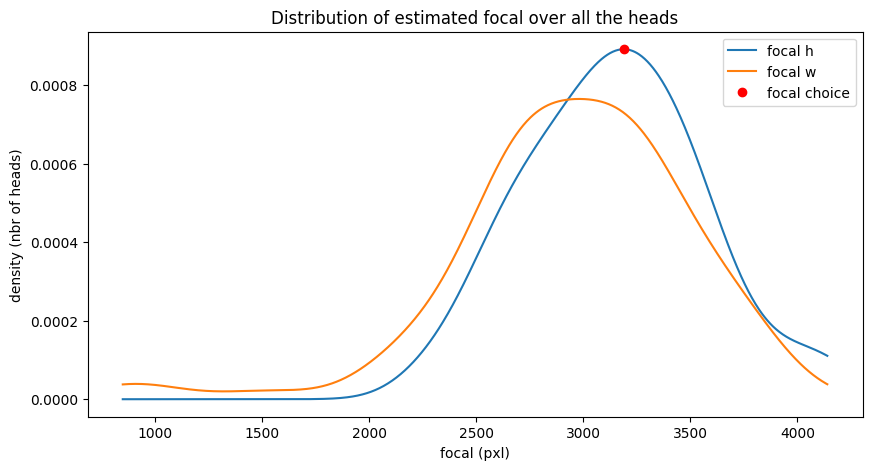
\includegraphics[width=0.45\textwidth]{images/focal_choice.png}
    \caption{Distribution des focales estimées pour chaque têtes, et choix de la valeur estimé de la focale (en pixels).}
    \label{fig:focal-estimation}
\end{figure}

Cette focale est très importante puisque c'est elle qui nous permet de calculer la ditance sur l'axe X en fonction de la profondeur (toujours grâce à la relationn \ref{eq:camera-relation}).